\documentclass[8pt]{extarticle}
\usepackage{amsmath}
\usepackage{amssymb}
\usepackage[utf8]{inputenc}
\usepackage{multicol}
\usepackage{mathtools}
\usepackage{graphicx}
\usepackage[swedish]{babel}
\usepackage[a4paper, margin=1.0cm]{geometry}
\title{Matematisk statistik TAMS27 formelblad}
\author{Mattias Salo}

\begin{document}
\maketitle
\begin{multicols*}{2}


\textbf{Väntevärde:}\\
\textit{Kontinuerlig}
\begin{equation*}
E[X] = \int_{-\infty}^{\infty} xf(x) dx
\end{equation*}
\textit{Diskret} ($\Omega$ är alla möjliga k)
\begin{equation*}
E[X] = \sum_{k \in \Omega} kP(X = k)
\end{equation*}

\textbf{Varians:}\\
\textit{Kontinuerlig}
\begin{equation*}
Var(X) = V(X) = \int_{-\infty}^{\infty} (x - E[X])^2 f_X(x)dx
\end{equation*}
förkortningsformel:
\begin{equation*}
Var(X) = E[X^2] - (E[X])^2 = \int_{-\infty}^{\infty} x^2 f_X(x)dx - (E[X])^2
\end{equation*}
\textit{Diskret}
\begin{equation*}
Var(X) = V(X) = \sum_{k \in \Omega} (k - E[X]^2P(X = k))
\end{equation*}
förkortningsformel:
\begin{equation*}
Var(X) = E[X^2] - (E[X])^2 = \sum_k k^2P(X=k) - (E[X])^2
\end{equation*}

\textbf{Standardavvikelse:}\\
\begin{equation*}
D(X) = \sqrt{Var(x)}
\end{equation*}

\textbf{Sats Räkneregler: (\textit{Diskret})}\\
a) $ E[a] = a, Var(a) = 0$ för varje icke slumpmässigt $a\in \mathbb{R}$\\
b) $E[aX + b] = a * E[X] + b ,$   $a, b \in \mathbb{R}$\\
$Var(aX + b) = a^2Var(X)$ (inget b på högra sidan)\\
c) Låt g vara en reell funktion. Det gäller att $E[g(X)] = \sum_k g(k)P(X = k)$\\

\textbf{Sats Räkneregler: (\textit{Kontinuerlig})}\\
a) och b) som i det diskreta fallet\\
c)Låt g vara en reell funktion. Det gäller att $E[g(X)]
= \int_{-\infty}^{\infty} g(x)f_X(x)dx.$\\
\\
\textbf{Simultana fördelningar:}\\
Låt $X,Y$ vara två kontinuerliga slumpvariabler.\\
\textit{Definition:}\\
a) $p(x, y) = P(X=x, Y=y)$ kallas \underline{simultan sannolikhetsfunktion} för (X,Y).\\
b)
\begin{equation*}
p_X(x) = P(X=x) = \sum_{y:p(x,y)>0}p(x,y)
\end{equation*}
\begin{equation*}
p_Y(y) = P(Y=y) = \sum_{x:p(x,y)>0}p(x,y)
\end{equation*}
kallas de \underline{marginella sannolikhetsfunktionerna}.\\
\underline{Anmärkning:}\\
Den marginella sannolikhetsfunktionen $p_X(x) = P(X=x)$ är samtidigt sannolikhetsfunktionen av s.v. $X$ om man inte tar hänsyn till $Y$.\\

Låt $X,Y$ vara två kontinuerliga slumpvariabler.\\
\textit{Definition:}\\
a) en funktion $f: \mathbb{R}^2 \longrightarrow [0,\infty)$ kallas \underline{simultan täthetsfunktion} av $(X,Y)$ om 
\begin{equation*}
P((X,Y) \in C) = \iint_{(x,y) \in C} f(x,y)dxdy
\end{equation*}
för varje $C \subseteq \mathbb{R}^2$.\\
b)
\begin{equation*}
f_X(x) = \int_{-\infty}^{\infty}f(x,y)dy, x\in\mathbb{R},
\end{equation*}
\begin{equation*}
f_Y(y) = \int_{-\infty}^{\infty}f(x,y)dx, y\in\mathbb{R},
\end{equation*}
kallas de \underline{marginella täthetsfunktionerna}.\\
\underline{Anmärkningar:}\\
(1) den marginella täthetsfunktionen $f_X(x)$ är samtidigt täthetsfunktionen av s.v. $X$ om man inte tar hänsyn till $Y$.\\
(2) Det gäller att 
\begin{equation*}
P(X \in A) = \int_{X \in A} \int_{y = -\infty}^{\infty} f(x,y) dydx = \int_{x \in A} f_X(x) dx, A \subseteq \mathbb{R}.
\end{equation*}

\textbf{Oberoende slumpvariabler}\\
\underline{definition}\\
Låt $X,Y$ vara två s.v. $X,Y$ kallas \underline{oberoende} om:
\begin{equation*}
P(X \in A, Y \in B) = P(X \in A) * P(Y \in B)
\end{equation*} 
för vilka två mängder som helst $A,B \subseteq \mathbb{R}$.\\
\underline{Sats:} a) Låt $X,Y$ vara två diskreta s.v.\\
$X,Y$ oberoende om och endast om 
\begin{equation*}
P(X = i, Y=j) = P(X = i) * P(Y = j)
\end{equation*}
för alla par $(i,j)$ som $(X,Y)$ kan anta. Detta skrivs också som $p(i,j) = p_X(i) * p_Y(j)$för alla par $(i,j)$.\\
b) Låt $X,Y$ vara två kontinuerliga s.v.\\
$X,Y$ är oberoende om och endast om 
\begin{equation*}
f(x,y) = f_X(x) * f_Y(y)
\end{equation*}
för alla $(x,y) \in \mathbb{R}^2$.\\
\\
\underline{Sats:} a) Låt $g: \mathbb{R}^2 \longrightarrow \mathbb{R}$. Det gäller att
\begin{equation*}
E[g(X,Y)] = 
	\begin{dcases}
		\sum_{alla}\sum_{(k,j)}g(k,j)p(k,j), X,Y diskreta\\
		\int_{-\infty}^{\infty}\int_{-\infty}^{\infty}g(x,y)f(x,y)dxdy, X,Y kontinuerliga
	\end{dcases}
\end{equation*}
där $p(k,j)$ är den gemensamma sannolikhetsfunktionen (diskret fall) och $f(x,y)$ är den gemensamma täthetsfunktionen (kontinuerligt fall).\\
b) Låt $X,Y$ vara oberoende och $g: \mathbb{R} \longrightarrow \mathbb{R}$, $h: \mathbb{R} \longrightarrow \mathbb{R}$. \\
Det gäller att: $E[g(X)*h(Y)] = E[g(X)] * E[h(Y)]$. \\
I synnerhet: $E[X*Y] = E[X] * E[Y]$.\\
\\
\underline{\textbf{Definition}}\\
$Cov(X,Y) = C(X,Y) = E[(X - E[X]) * (Y - E[Y])]$.\\
kallas \underline{kovarians} av $X$ och $Y$.\\
\underline{Anmärkningar}: (1) Fördelaktigt: Förkortningsformeln:\\
$Cov(X,Y) = E[X*Y] - E[X] * E[Y]$\\
(2) I synnerhet, om $X$ och $Y$ är oberoende $Cov(X,Y) = 0$.\\
(3) Motriktningen kan vara fel.\\

\underline{Sats} (räkneregler för Cov)\\
(1) $Cov(X,X) = Var(X)$\\
(2) $Cov(X,Y) = Cov(Y,X)$\\
(3) $Cov(aX,Y) = Cov(X,aY) = a * Cov(X,Y), a \in \mathbb{R}$\\
(4) $Cov(\sum_{i = 1}^mX_i, \sum_{j = 1}^nY_j) = \sum_{i = 1}^m \sum_{j = 1}^n Cov(X_i, Y_j)$\\
\underline{Följdsats}:\\
(1) $Cov(a, X) = Cov(X, a) = 0, a \in \mathbb{R}$\\
(2) $Cov(\sum_{i = 1}^ma_iX_i+b, \sum_{j = 1}^nc_jY_j+d) = \sum_{i = 1}^m \sum_{j = 1}^n a_ic_j Cov(X_i, Y_j)$\\
(3) $Var(\sum_{i = 1}^m X_i) = \sum_{i = 1}^m Var(X_i) + \sum_{i \neq j} Cov(X_i, X_j)$\\
\\
\underline{\textbf{Definition}}:\\
\begin{equation*}
\rho (X,Y) = \frac{Cov(X,Y)}{\sqrt{Var(X) * Var(Y)}}
\end{equation*}
kallas \underline{korrelation} mellan $X$ och $Y$.\\
\underline{Sats} a) $|\rho(X,Y)| \leq Var(X)Var(Y)$\\
b) $|\rho(X,Y)| = 1$ om och endast om det finns $a,b,c \in \mathbb{R}$ sådana att $aX + BY = c$.\\
\underline{Anmärkning} a) är ekvivalent med\\
$(Cov(X,Y))^2 \leq Var(X)*Var(Y)$\\
den stokastiska versionen av Schwarz' olikhet.\\

\textbf{Centrala gränsvärdessatsen}:\\
Låt $X_1,X_2,..."$ vara en oändlig följd av oberoende och likafördelade stokastiska variabler med väntevärde $\mu$ och med standardavvikelsen $\sigma > 0$. Låt den stokastiska variabeln
\begin{equation*}
Y_n = X_1 + X_2 + ... + X_n
\end{equation*}
beteckna summan av de första $n$ stokastiska variablerna i följden.\\
Då gäller att
\begin{equation*}
\lim_{n \rightarrow \infty} P\left( a < \frac{Y_n - n\mu}{\sigma \sqrt{n}} \leq b \right) = \Phi (b) - \Phi (a)
\end{equation*}
där $\Phi (a)$ betecknar fördelningsfunktionen för en standardiserad normalfördelning.\\
\\
\textbf{Normalfördelning}:\\
Normalfördelningen har täthetsfunktionen
\begin{equation*}
f(x) = \frac{1}{\sigma\sqrt{2 \pi}} e^{-\frac{(x - \mu)^2}{2 \sigma^2}}
\end{equation*}
där $\mu$ och $\sigma$ är normalfördelningens karakteristiska konstanter: $\mu$ är väntevärdet och $\sigma$ är standardavvikelsen för fördelningen. Denna normalfördelning betecknas med $N(\mu,\sigma)$.\\
Normalfördelningens täthetsfunktion kan inte integreras med vanliga endimensionella metoder eftersom den inte har någon primitiv funktion som kan uttryckas analytiskt. Arean under kurvan kan emellertid med andra metoder visas vara 1, vilket den måste vara för att vara en sannolikhetsfördelning.\\
En \textbf{standardiserad normalfördelning} har $\mu$ = 0 och $\sigma$ = 1.\\
Fördelningsfunktionen för en standardiserad normalfördelning brukar betecknas med $\Phi$, och sambandet mellan fördelningsfunktion och täthetsfunktion är
\begin{equation*}
\Phi (x) = \int_{-\infty}^x f(z)dz.
\end{equation*}
Fördelningsfunktionen anger sannolikheten för att en normalfördelad variabel Y är mindre än eller lika med ett visst tal a:
\begin{equation*}
P(Y < a) = \Phi	(a).
\end{equation*}
Sannolikheten att en normalfördelad variabel Y hamnar i ett intervall $[a,b]$ är
\begin{equation*}
P(a < Y < b) = \Phi (b) - \Phi (a).
\end{equation*}
\textbf{Fördelningsfunktion}\\
Fördelningsfunktionen för en godtycklig normalfördelad variabel $X \in N(\mu , \sigma)$  kan erhållas från fördelningsfunktionen för en standardnormalfördelad variabel:
\begin{equation*}
P(X < a) = \Phi \left(\frac{a - \mu}{\sigma}\right).
\end{equation*}
\begin{equation*}
P(a < X < b) = \Phi \left(\frac{b - \mu}{\sigma}\right) - \Phi \left(\frac{a - \mu}{\sigma}\right).
\end{equation*}
Denna egenskap medför att tabeller för normalfördelningar bara redovisar fördelningsfunktionen $\Phi$, eftersom alla andra normalfördelningar på detta sätt kan översättas till en normalfördelning med väntevärdet 0 och standardavvikelsen 1.\\
\underline{Sats}: Om $X_1, ... , X_n$ är oberoende $N(\mu,\sigma)$ och $\overline{X} = \sum_1^nX_i / n$ är deras aritmetiska medelvärde, så gäller att: $\overline{X} \in N(\mu, \sigma/\sqrt{n})$.\\
\\
\textbf{Markovkedjor}:\\
Irreducibel är att alla noder går att nå från alla. Aperiodisk är när en nod kan gå till sig själv. Om den både är irreducibel och aperiodisk är den ergodisk.\\
\\
\textbf{Lagen om total sannolikhet}:\\
Det då jag skriver ett träd är lagen om total sannolikhet.\\
\textbf{Bayes' sats}:\\
Låt $A_1, ... , A_n$ vara $n$ disjunkta (oförenliga) händelser med positiv sannolikhet. Anta att Händelserna utgör hela utfallsrummet $\cup_{i=1}^n A_i = \Omega$. Bayes' sats säger då att 
\begin{equation*}
P(A_i|B) = \frac{P(Ai)P(B|A_i)}{\sum_{j=1}^nP(A_j)P(B|A_j)}
\end{equation*}
där nämnaren är lika med $P(B)$ enligt lagen om total sannolikhet.\\
För specialfallet $n=1$ ger Bayes sats
\begin{equation*}
P(A|B)=\frac{P(A)P(B|A)}{P(B)}
\end{equation*}
Där $P(A|B)$ är sannolikheten för $A$, givet $B$.\\
\\
\textbf{Betingad sannolikhet}
\begin{equation*}
P(B|A) = \frac{P(A \cap B)}{P(A)}
\end{equation*}
\\
Om en Poissonfördelning används och du skall räkna ut en sannolikhet över flera händelser kan du multiplicera antalet händelser med det originella $\mu$-värdet.\\
$X \sim Po(\mu)$ och $Y = X_1,X_2,...,X_n$ kan det sägas att $Y \sim Po(n * \mu)$.\\
\\
\textbf{Markovkedjor}\\
\underline{definition}: a) Låt $X_0,X_1,...$ vara en följd av stokastiska variabler som kan anta värdena $0,1,2,...,M$. Man säger att systemet är vid tid n i tillståndet $i \in {0,1,...,M}$ om $X_n = i$.
\begin{center}
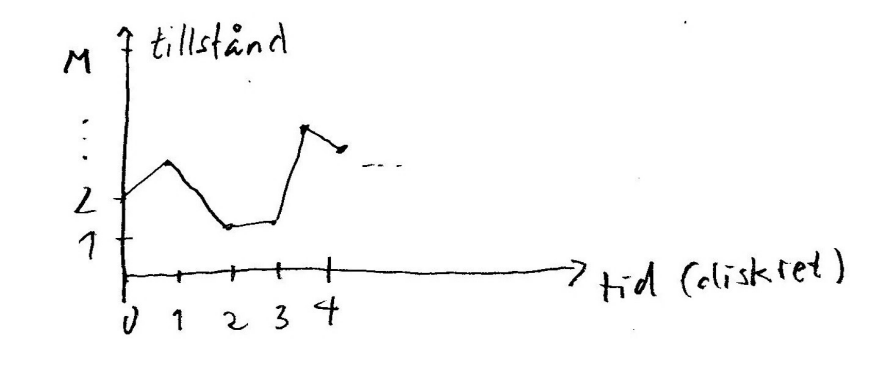
\includegraphics[width=\linewidth]{markov.png}
\end{center}
b) Följden $X_0,X_1,...$ bildar en \underline{Markovkedja} om varje gång när systemet är i tillstånd $i \in {0,1,...,M}$ finns det en sannolikhet $p_{ij}$ att systemet kommer att vara i tillstånd j näst. Dvs för alla $i_0,...,i_{n-1},i,j$.
\begin{equation*}
p_{ij} = P(X_{n+1} = j | X_n = i, X_{n-1} = i_{n-1}, ..., X_0 = i_0)
\end{equation*}
c) Värdena $p_{ij}$, $0 \leq i , j \leq M$, kallas \underline{övergångssannolikhet}. Matrisen $p = [p_{ij}]_{ij} = 0, ..., M$ kallas \underline{övergångsmatris}.\\
\underline{Anmärkning} $P(X_{n+1} = j | X_n = i, X_{n-1} = i_{n-1}, ... , X_0 = i_0) = p_{ij} = P(X_{n+n} = j | X_n = i)$ \underline{Markovprincipen}.\\
\underline{Sats} (Chapman-Kolmogorov ekvationer), Låt $p_{ij}^{(n)}$ vara sannolikheten att systemet är i tillstånd $i$ och kommer att vara i tillstånd $j$ efter $n$ steg (tidsenheter). Det gäller att
\begin{equation*}
p_{ij}^{(n)} = \sum_{k=0}^M p_{ik}^{(r)} * p_{kj}^{(n-r)}
\end{equation*}
för alla $0<r<n$.\\
\underline{Anmärkningar} 1) Låt
\begin{equation*}
P^{(n)} = [p_{ij}^{(n)}]_{i,j = 0,...,M}
\end{equation*}
beteckna \underline{n-steg övergångsmatrisen}\\
Satsen kan skrivas som $$P^{(n)} = p^{(r)} * p^{(n-r)}$$ (matrismultiplikation)\\
2) I synnerhet $p=p^{(1)}$ och $$p^{(n)} = p*..*p=p^n$$ (matrispotens)

\end{multicols*}
\end{document}